\documentclass[11pt,a4paper]{article}
\usepackage[T1]{fontenc}
\usepackage[utf8]{inputenc}
\usepackage[romanian]{babel}
\usepackage{amsmath,amssymb}
\usepackage{graphicx}
\usepackage{booktabs}
\usepackage{geometry}
\usepackage{hyperref}
\usepackage{caption}
\usepackage{float}
\geometry{margin=2.5cm}

\title{De ce se mișcă Bursa de la București?\\ Măsurarea vitezei și calibrarea magnitudinii șocurilor politice, 2020--2026}
\author{}
\date{septembrie 2026}

\begin{document}
\providecommand{\NullSd}{1{,}94}
\providecommand{\NullPqfive}{3{,}98}
\providecommand{\NullMax}{9{,}81}
\providecommand{\NullFreqThree}{10{,}2}
\providecommand{\TurTwoCar}{6{,}94}
\providecommand{\TurTwoP}{0{,}014}
\providecommand{\TurTwoPct}{98{,}8}
\providecommand{\ParlCar}{-3{,}74}
\providecommand{\ParlP}{0{,}066}
\providecommand{\TurOneCar}{-3{,}50}
\providecommand{\TurOneP}{0{,}076}
\providecommand{\CiucaCar}{-2{,}60}
\providecommand{\CiucaP}{0{,}132}
\providecommand{\CiucaT}{-3{,}02}
\providecommand{\CiucaStoxx}{-3{,}67}
\providecommand{\CiucaBet}{-3{,}41}
\providecommand{\CiucaInvestDay}{0{,}57}
\providecommand{\LocaleBet}{-3{,}01}
\providecommand{\LocaleTr}{-0{,}59}
\providecommand{\LocaleT}{-3{,}49}
\providecommand{\CcrCar}{4{,}34}
\providecommand{\CcrP}{0{,}038}
\providecommand{\CcrArZero}{2{,}97}
\providecommand{\FitchCar}{-4{,}31}
\providecommand{\FitchP}{0{,}040}
\providecommand{\NegMean}{-1{,}00}
\providecommand{\NegN}{7}
\providecommand{\TrioMean}{-2{,}94}
\providecommand{\TlvMay}{-4{,}11}
\providecommand{\BetMay}{-2{,}88}
\providecommand{\BetFiMay}{-4{,}51}
\providecommand{\NEvents}{24}
\providecommand{\AggP}{0{,}026}
\providecommand{\AggPerm}{20000}
\providecommand{\EvMeanAbs}{2{,}00}
\providecommand{\NullMeanAbs}{1{,}38}
\providecommand{\AggObs}{3}
\providecommand{\AggExp}{1{,}1}
\providecommand{\AggN}{22}
\providecommand{\RhoWindow}{1{,}000}
\providecommand{\PqPostCovid}{4{,}00}
\providecommand{\NPfivePostCovid}{3}

\maketitle

\begin{abstract}
\noindent\textbf{Întrebarea.} Cât de repede și cât de puternic reacționează acțiunile de la
Bursa de Valori București la știrile politice? Am aplicat un event-study pe \NEvents{}
evenimente din 2020--2026, pe cotații zilnice ale indicelui BET, a 8 acțiuni lichide și a
4 indici complementari, plus bare intraday la 15 minute în jurul celor trei șocuri
electorale mari.

\noindent\textbf{Viteza.} Reacția la șocurile electorale se formează la deschiderea
primei ședințe de după eveniment. În noiembrie 2024 minimul zilei a fost atins la 15 minute
de la deschidere.

\noindent\textbf{Magnitudine, în două sensuri.} Am calibrat rezultatele cu un test placebo de
500 de pseudo-evenimente, aplicate aceluiași estimator. Distribuția nula a randamentului
anormal cumulat pe trei ședințe are $\sigma = \NullSd\%$, iar $|CAR_3|$ la percentila 95 este
$\NullPqfive\%$: o mișcare de 3\% peste trei ședințe se produce la BVB în $\NullFreqThree\%$ din
cazuri, fără nicio știre politică. Privite unul câte unul, doar trei dintre cele \NEvents{}
evenimente trec pragul de 5\% (victoria din turul al doilea, $\TurTwoCar\%$, $p = \TurTwoP$,
care se separă cel mai clar). Privite în ansamblu, însă, evenimentele politice se departă
semnificativ de zgomotul obișnuit: modulul mediu al mișcării pe zile de eveniment este
$\EvMeanAbs\%$ față de $\NullMeanAbs\%$ pe zile oarecare, cu $p = \AggP$ într-un test de
permutare, iar $\AggObs$ evenimente trec percentila 95 față de $\AggExp$ așteptate doar din
șansă.

\noindent\textbf{Secțional.} Șocurile electorale mari sunt interne: STOXX Europe 600 a fost
plat sau ușor pozitiv în zilele-cheie, în timp ce BET a divergit tare. Băncile absorb prima
lovitură (TLV $\TlvMay\%$ într-o singură zi).

\noindent\textbf{Contribuție secundară, de metodă.} Trei dintre cele mai spectaculoase
rezultate ale unui event-study obișnuit s-au dovedit a fi eșecuri de măsură, nu fenomene de
piață: o fereastră de estimare fixă prinsă într-un regim liniștit umflă toate statisticile t
simultan; parametrul de ajustare al fluxului public BVB nu corectează dividendele; iar un
control de piață calibrat într-o perioadă calmă poate transforma o zi de cădere globală
într-un efect domestic fictiv.
\end{abstract}

\begin{abstract}
\noindent\textbf{Question.} How fast and how strongly do Bucharest Stock Exchange shares
react to political news? We apply an event study to \NEvents{} events over 2020--2026, using
daily quotes for the BET index, 8 liquid stocks and 4 complementary indices, plus
15-minute bars around the three major electoral shocks.

\noindent\textbf{Speed.} Reactions to electoral shocks form at the open of the first session
after the event; in November 2024 the intraday low came 15 minutes after the open.

\noindent\textbf{Magnitude, in two senses.} Results are calibrated with a placebo test of 500
pseudo-events run through an identical estimator. The null distribution of three-day
cumulative abnormal returns has $\sigma = \NullSd\%$ and a 95th percentile of
$\NullPqfive\%$, so a 3\% move over three days occurs on roughly $\NullFreqThree\%$ of BVB
sessions with no political news at all. Read one at a time, only three of the \NEvents{}
events clear the 5\% threshold (the second-round presidential victory, $\TurTwoCar\%$,
$p = \TurTwoP$, being the clearest). Read in aggregate, however, political events do depart
significantly from ordinary noise: mean absolute movement on event days is $\EvMeanAbs\%$
against $\NullMeanAbs\%$ on ordinary days, $p = \AggP$ in a permutation test, with
$\AggObs$ events above the 95th percentile against $\AggExp$ expected by chance alone.

\noindent\textbf{Robustness.} Re-running the placebo test with four different estimation
windows (40 to 250 sessions) leaves the ranking of events unchanged (rank correlation
$\RhoWindow$), and restricting the null to the post-COVID regime gives a 95th percentile of
$\PqPostCovid\%$, essentially the same as the full period: the fat tails are not an artifact
of the pandemic.

\noindent\textbf{Cross-section.} The large electoral shocks are domestic: STOXX Europe 600
was flat or slightly positive on the event days while BET diverged sharply. Banks absorb the
first blow (TLV $\TlvMay\%$ in a single day).

\noindent\emph{Secondary, methodological contribution.} Three of the most eye-catching
results of an ordinary event study turn out to be measurement failures rather than market
phenomena: a fixed estimation window that lands in a calm regime inflates every t-statistic
at once; the public BVB feed's adjustment flag does not correct for dividends; and a market
control estimated in calm conditions can turn a global crash day into a fictitious domestic
effect.
\end{abstract}

\section{Date și Metodă}

\subsection{Cotații}

Bursa de Valori București nu publică un API pentru dezvoltatori, dar site-ul propriu rulează
un flux de date compatibil TradingView la \url{https://wapi.bvb.ro/api}, care răspunde la
cereri HTTP simple. Parametrii sunt \texttt{symbol}, \texttt{from}, \texttt{to},
\texttt{rs}, \texttt{ajust}, \texttt{countback} și \texttt{currencyCode}; rezoluția zilnică
se cere ca \texttt{rs=1D}. Am descărcat bare zilnice în RON pentru 1 ianuarie 2020 --
28 septembrie 2026: indicele BET, 8 acțiuni lichide (TLV, SNP, BRD, H2O, SNG, DIGI, TEL,
SNN) și 4 indici complementari (ROTX, BET-TR, BET-FI, BET-NG), aproximativ 1.690 de
ședințe per simbol. H2O intră în serie abia din iulie 2023, la listarea celui mai mare IPO
din istoria bursei. Pentru măsurarea vitezei am descărcat și bare la 15 minute pentru BET și
TLV în jurul celor trei șocuri majore.

O limită a sursei schimbă rezultatele, deci o semnalăm aici. Parametrul \texttt{ajust}
corectează doar spliturile, nu dividendele. Verificarea este directă: randamentul TLV din
11.06.2024, $-4{,}69\%$, este identic în seria ajustată și în cea neajustată. Randamentele de
preț sunt așadar contaminate în ferestrele de ex-dividend, iar sezonul de dividende al
băncilor românești, în iunie, cade în mijlocul ferestrei analizate. Seria primară este
deci \textbf{BET-TR}, indicele de randament total al bursei, care nu suferă de acest efect.
Paralel, pipeline-ul marchează automat orice eveniment la care diferența dintre BET și BET-TR
depășește un punct procentual pe aceeași fereastră.

\subsection{Benchmark și evenimente}

Ca model al pieței europene am folosit STOXX Europe 600, descărcat zilnic prin interfața
publică de grafice Yahoo Finance și aliniat pe calendarul burseui prin reportarea ultimei
valori disponibile.

Articolele din fluxurile RSS ale G4Media, HotNews, Digi24 și Economica au fost colectate
automat și filtrate pe cuvinte-cheie politice. RSS-ul acoperă însă doar prezentul, deci baza
istorică este un tabel de \NEvents{} evenimente datate manual, fiecare cu nivel de
încredere și o clasificare \emph{ex-ante}: origine (intern, extern, piață) și semn așteptat.
Tabelul~\ref{tab:events} le listează.

\subsection{Estimator}

Fereastra de estimare este $[-60,-11]$ ședințe de tranzacționare, trunchiată la începutul
seriei, cu minim 30 de observații. Ferestrele de eveniment sunt $[0,0]$, $[-1,+1]$ și
$[-5,+5]$. Pentru BET și indici, randamentul anormal este $AR_t = R_t - \bar{R}_{est}$.
Pentru acțiuni folosim modelul de piață OLS față de BET, iar pentru controlul extern modelul
OLS al BET față de STOXX 600, ambii estimați pe perioada de estimare. Statistica uzuală este
$t = CAR / (\hat{\sigma}\sqrt{T})$.

Ziua 0 este ședința în care apare știrea dacă aceasta cade înainte de ora 18:00, și
următoarea ședință de tranzacționare în caz contrar. Toate scrutinurile au avut loc duminica
seara, deci ziua 0 este lunea, iar prețul de deschidere prinde integral informația acumulată
în weekend.

\subsection{Calibrarea cu test placebo}

Statisticile t de mai sus presupun randamente normale și independente, cu volatilitatea
măsurată în fereastra de estimare. La o piață mică și ilichidă această presupunere e
problematică: o fereastră fixă de 50 de ședințe poate cădea într-un regim liniștit și poate
subestima volatilitatea folosită ca denominator. Pentru a elimina dependența de un parametru
alegut de noi, calibrăm cu un test placebo. Trasăm 500 de ședințe pseudo-aleatoare,
excluzând câte trei ședințe în jurul fiecărui eveniment real, și aplicăm același estimator.
Distribuția obținută arată cât de mare este un CAR obișnuit la BVB, iar fiecare eveniment
primește o valoare p empirică bilaterată pe $|CAR|$.

\section{Rezultate}

\subsection{Viteza: reacția se formează la deschidere}

Tabelul~\ref{tab:speed} și Figura~\ref{fig:intra} rezumă barele la 15 minute. Pe 25
novembrie 2024 gap-ul la deschidere a fost $-1{,}57\%$, minimul zilei, $-1{,}84\%$, a fost
atins la 10:15, iar închiderea a recuperat la $-0{,}89\%$. Pe 5 mai 2025 gap-ul de
$-2{,}13\%$ s-a adâncit continuu până la închidere. Pe 19 mai 2025, în sens pozitiv,
aproape tot câștigul s-a format la deschidere.

\begin{table}[H]
\centering
\caption{Viteza reacției intraday a indicelui BET, din bare la 15 minute.}
\label{tab:speed}
{\footnotesize\setlength{\tabcolsep}{3.5pt}
\begin{tabular}{p{4.4cm}rrr p{3.4cm}}
\toprule
Shock & Opening gap & Intraday low (local) & Close & Pattern \\
\midrule
Presidential first round 2024 & $-1{,}57\%$ & $-1{,}84\%$ (10:15) & $-0{,}89\%$ & instant shock, partial recovery \\
Presidential first round 2025 & $-2{,}13\%$ & $-2{,}88\%$ (17:45) & $-2{,}88\%$ & degraded all day \\
Presidential second round 2025 & $4{,}12\%$ & $3{,}62\%$ (12:30) & $4{,}08\%$ & instant gain \\
\bottomrule
\end{tabular}}

\end{table}

\begin{figure}[H]
\centering
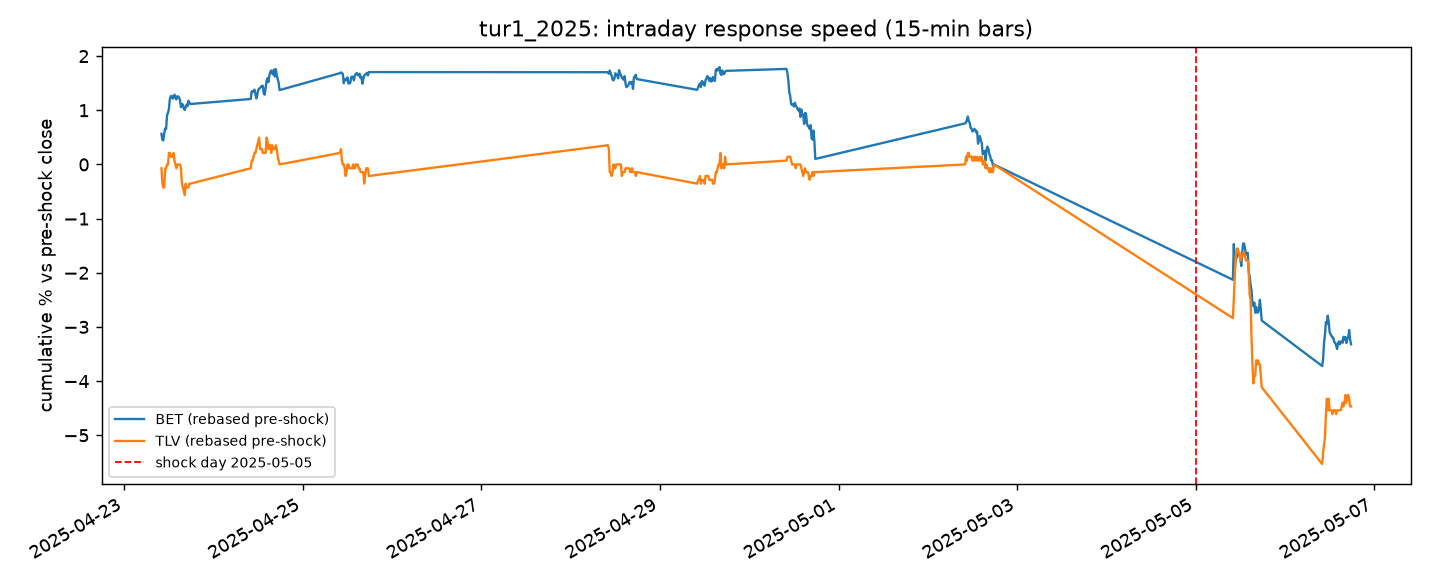
\includegraphics[width=\textwidth]{../outputs/fig_intraday_tur1_2025.png}
\caption{Reacția intraday la turul întâi din mai 2025. BET și TLV rebazate la închiderea dinaintea șocului.}
\label{fig:intra}
\end{figure}

\subsection{Cine reacționează mai tare}

Tabelul~\ref{tab:idx} compară indicii pe fereastra de trei ședințe. ROTX reproduce BET,
ceea ce exclude o anomalie de construcție a indicelui. Sectorul financiar amplifică panica din
mai 2025, cu $\BetFiMay\%$ față de BET, iar energia amortizează sistematic, cu
$-2{,}82\%$ față de $-3{,}50\%$. La nivelul acțiunilor, băncile absorb prima lovitură: TLV a
căzut $\TlvMay\%$ pe 5 mai 2025, față de $\BetMay\%$ pentru BET.

\begin{table}[H]
\centering
\caption{CAR$[-1,+1]$ pe indici, în procente. Seria primară este BET-TR.}
\label{tab:idx}
\begin{tabular}{lrrrr}
\toprule
Eveniment & BET-TR & ROTX & BET-FI & BET-NG \\
\midrule
tur1 2024 & $-1{,}60$ & $-1{,}28$ & $0{,}03$ & $-0{,}90$ \\
parlamentare 2024 & $-3{,}74$ & $-3{,}58$ & $-3{,}55$ & $-2{,}87$ \\
ccr anulare 2024 & $4{,}34$ & $4{,}21$ & $1{,}90$ & $3{,}67$ \\
tur1 2025 & $-3{,}50$ & $-3{,}32$ & $-4{,}51$ & $-2{,}82$ \\
tur2 2025 & $6{,}94$ & $6{,}88$ & $5{,}14$ & $6{,}13$ \\
\bottomrule
\end{tabular}

\end{table}

\begin{figure}[H]
\centering
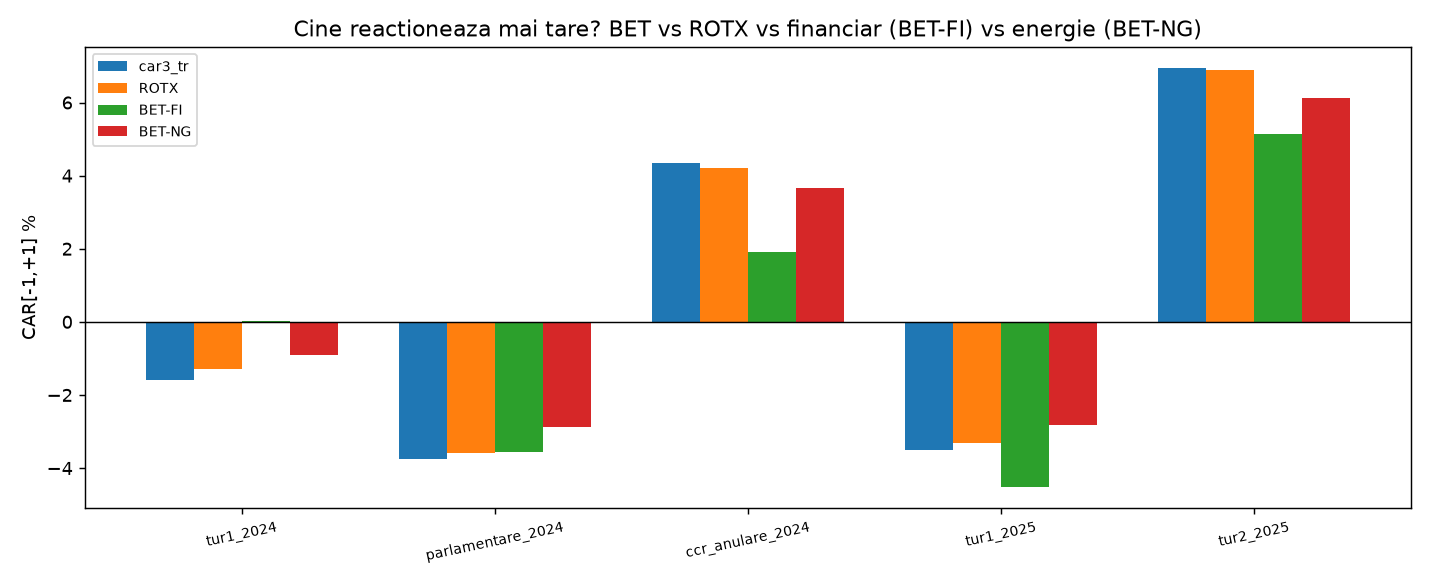
\includegraphics[width=\textwidth]{../outputs/fig_indices_car3.png}
\caption{CAR$[-1,+1]$ pe indici la cele cinci șocuri majore.}
\label{fig:idx}
\end{figure}

\subsection{Șocurile electorale mari sunt interne}

În zilele-cheie, STOXX Europe 600 este practic plat: $+0{,}06\%$ pe 25 noiembrie 2024,
$+0{,}16\%$ pe 5 mai 2025 și $+0{,}13\%$ pe 19 mai 2025. În aceleași zile BET înregistrează
$-0{,}89\%$, $-2{,}88\%$ și $+4{,}08\%$. Divergențele sunt, așadar, domestice.

\begin{figure}[H]
\centering
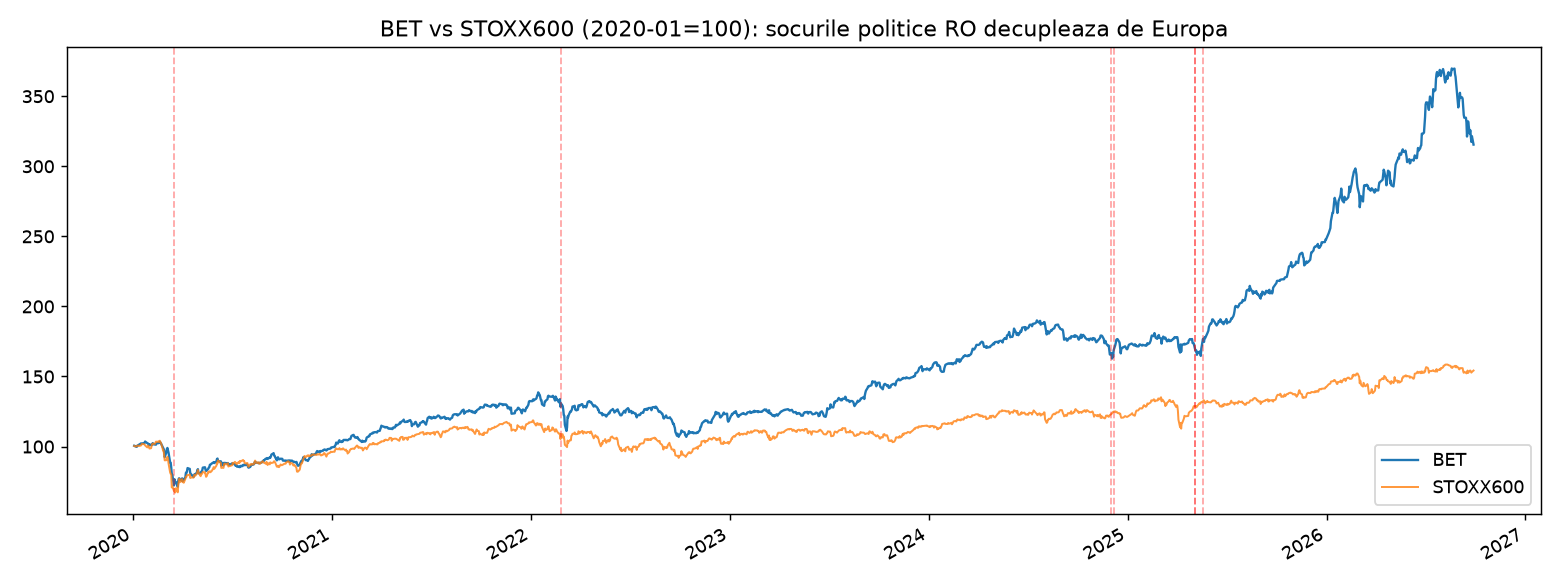
\includegraphics[width=\textwidth]{../outputs/fig_bet_vs_stoxx.png}
\caption{BET și STOXX 600, baza 100 la începutul lui 2020. Liniile verticale marchează șocurile politice cu încredere ridicată.}
\label{fig:stoxx}
\end{figure}

\subsection{Calibrarea placebo}

Testul placebo produce cel mai important rezultat al lucrării, pentru că recalibrează
lectura tuturor celorlalte. Distribuția nula a CAR$[-1,+1]$ are media $-0{,}03\%$ și
$\sigma = \NullSd\%$, cu $|CAR_3|$ la percentila 95 de $\NullPqfive\%$ și maximul de
$\NullMax\%$. La BVB, o mișcare de 3\% peste trei ședințe apare în $\NullFreqThree\%$ din
ședințe fără nicio știre politică. Pragul efectiv de detectabilitate al unui eveniment
politic este de ordinul a 4\%.

\begin{table}[H]
\centering
\caption{Test placebo: CAR$[-1,+1]$ pe BET-TR, comparat cu distribuția nula.}
\label{tab:placebo}
{\footnotesize\setlength{\tabcolsep}{4pt}
\begin{tabular}{lrrrl}
\toprule
Eveniment & CAR$_3$ & $t$ clasic & $p$ empiric & Verdict placebo \\
\midrule
tur2 2025 & $6{,}94$ & $3{,}58^{**}$ & $0{,}014$ & se separă de null \\
ccr anulare 2024 & $4{,}34$ & $3{,}91^{**}$ & $0{,}038$ & se separă de null \\
fitch negativ 2024 & $-4{,}31$ & $-3{,}10^{**}$ & $0{,}040$ & se separă de null \\
parlamentare 2024 & $-3{,}74$ & $-3{,}71^{**}$ & $0{,}066$ & marginal \\
demisie ciolacu 2025 & $-3{,}50$ & $-1{,}80$ & $0{,}076$ & marginal \\
tur1 2025 & $-3{,}50$ & $-1{,}80$ & $0{,}076$ & marginal \\
guvern ciolacu2 2024 & $2{,}97$ & $1{,}82$ & $0{,}108$ & nesemnificativ \\
\bottomrule
\end{tabular}}

\end{table}

Dintre \NEvents{} evenimente politice din șase ani și jumătate, trei trec pragul de 5\%:
victoria din turul al doilea al prezidențialelor din mai 2025, cu $\TurTwoCar\%$ și
$p = \TurTwoP$ (percentila $\TurTwoPct$), anularea alegerilor de către CCR
($\CcrCar\%$, $p = \CcrP$) și revizuirea perspectivei de către Fitch
($-\FitchCar\%$, $p = \FitchP$). Parlamentarele din decembrie 2024, la $p = \ParlP$, rămân
în interiorul distribuției normale, deși testul t clasic le-ar fi raportat drept
semnificative.

\subsection{Testul agregat: mișcă știrile politice piața, în ansamblu?}

Testele per eveniment suferă de multiplicitate: cu \NEvents{} evenimente și un prag de 5\%,
aproape unul ar trece din întâmplare. Testul agregat evită problema, fiindcă pune întrebarea
direct: \emph{este modulul mediu al mișcării mai mare în zilele de eveniment decât în zilele
obișnuite?}

Pe cele \AggN{} ședințe distincte de eveniment, modulul mediu al lui $|CAR|$ este
$\EvMeanAbs\%$, față de $\NullMeanAbs\%$ pe zile fara eveniment. Am comparat prin
\AggPerm{} de permutări aleatoare din nulla, iar diferența are $p = \AggP$. Trei evenimente
trec percentila 95, față de $\AggExp$ câte ar fi așteptate doar din șansă. Concluzia, în
forma în care rezistă testelor: știrile politice produc la BVB mișcări mai mari decât zgomotul
de fond, dar fiecare eveniment luat separat are o marjă de eroare prea mare pentru a fi
distins de zgomot.

\begin{figure}[H]
\centering
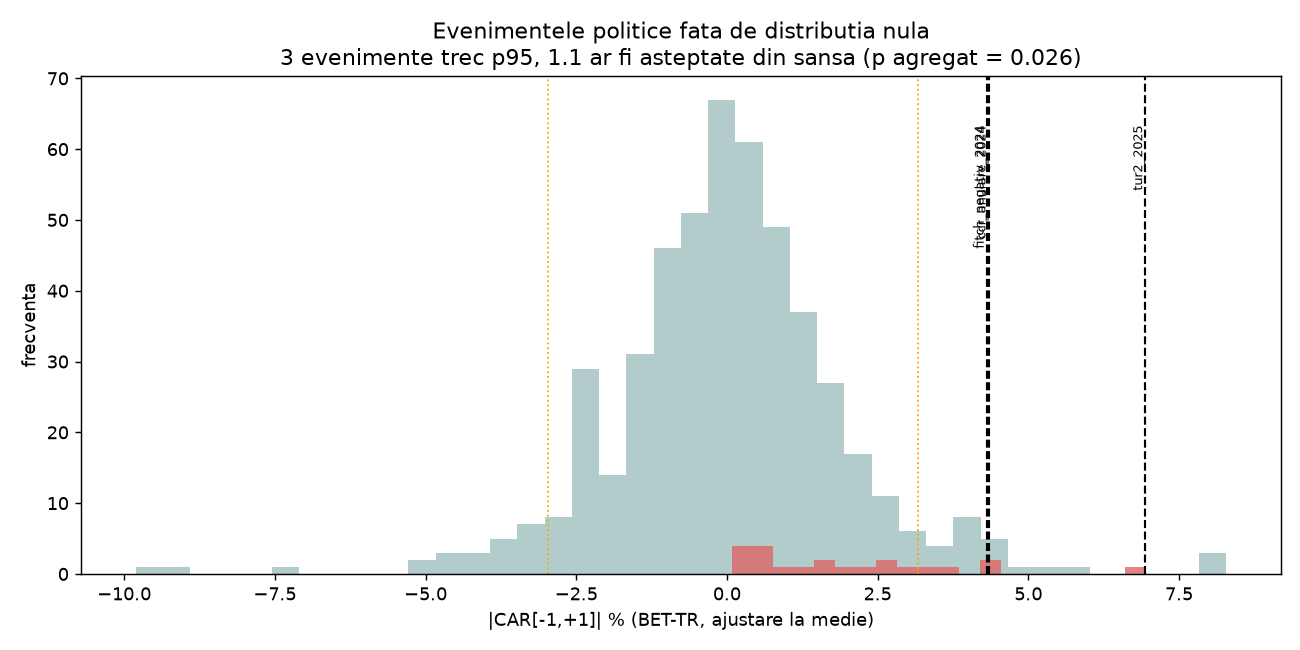
\includegraphics[width=\textwidth]{../outputs/fig_placebo.png}
\caption{Modulul mișcării pe zile de eveniment politic față de distribuția nula a zilelor fără eveniment.}
\label{fig:placebo}
\end{figure}

\subsection{Sensibilitate: depinde concluzia de fereastra de estimare?}

Fereastra de estimare $[-60,-11]$ a fost o alegere arbitrară, iar toată problema identificată
mai sus provine din faptul că poate prinde un regim neobișnuit. Tabelul~\ref{tab:window}
reia întregul test placebo cu patru ferestre, de la 40 la 250 de ședințe înaintea
evenimentului.

\begin{table}[H]
\centering
\caption{Rezultatele placebo în funcție de fereastra de estimare.}
\label{tab:window}
{\footnotesize\setlength{\tabcolsep}{4pt}
\begin{tabular}{lrl p{9.6cm}}
\toprule
Estimation window & $n$ & $p<0{,}05$ & Events \\
\midrule
$[-250,\;10]$ & 19 & 4 & Presidential second round 2025, Constitutional Court annulment 2024, Fitch outlook to negative 2024, Parliamentary elections 2024 \\
$[-120,\;10]$ & 19 & 4 & Presidential second round 2025, Constitutional Court annulment 2024, Fitch outlook to negative 2024, Parliamentary elections 2024 \\
$[-60,\;10]$ & 19 & 4 & Presidential second round 2025, Constitutional Court annulment 2024, Fitch outlook to negative 2024, Parliamentary elections 2024 \\
$[-40,\;10]$ & 19 & 4 & Presidential second round 2025, Constitutional Court annulment 2024, Fitch outlook to negative 2024, Parliamentary elections 2024 \\
\bottomrule
\end{tabular}}

\end{table}

Identificarea evenimentelor care trec pragul nu se schimbă deloc, iar corelația de rang între
ferestre este $\RhoWindow$, adică concluzia nu depinde de alegerea fereștrii. Doi factori
merită totuși precizate. Numărul evenimentelor care ating 5\% crește de la trei la patru
când fereastra se lungeste, fiindcă percentila 95 a nullei scade de la $\NullPqfive\%$ la
aproximativ $3{,}4\%$. Iar calculul pe regimul post-COVID, excluzândRestrictionile din 2020
și 2021, dă o percentilă 95 de $\PqPostCovid\%$, practic aceeași cu cea pe întreaga perioadă:
cozile groase ale distribuției nu sunt un artefact al pandemiei.

Explicația este una singură și verificabilă. Fereastra fixă de estimare capturează un regim
liniștit, subestimează volatilitatea reală folosită ca denominator și umflă $|t|$ pentru toate
evenimentele simultan. Placebo-ul este imun prin construcție, fiindcă eșargește din întreaga
perioadă. Concluzia nu este că știrile politice nu contează, ci că la dimensiunea și
lichiditatea acestei piețe pragul la care un eveniment politic devine vizibil depășește ce
poate raporta onest un test standard.

Tabelul~\ref{tab:main} arată aceleași evenimente în formatul clasic, pe care placebo-ul îl
recalibrează.

\begin{table}[H]
\centering
\caption{Efectele brute ale evenimentelor majore, cu statisticile $t$ clasice.}
\label{tab:main}
{\footnotesize\setlength{\tabcolsep}{3pt}
\begin{tabular}{lrrrrr}
\toprule
Event & Day $0$ & $AR_0$ & CAR$[-1,+1]$ & CAR$[-5,+5]$ & Net STOXX \\
\midrule
Presidential first round 2024 & 25 Nov & $-0{,}80$ & $-1{,}59$ & $-5{,}99$ & $-1{,}86$ \\
Parliamentary elections 2024 & 2 Dec & $0{,}60$ & $-3{,}73^{**}$ & $-0{,}91$ & $-3{,}93$ \\
Constitutional Court annulment 2024 & 6 Dec & $2{,}97^{**}$ & $4{,}35^{**}$ & $4{,}66$ & $4{,}22$ \\
Presidential first round 2025 & 5 May & $-2{,}91^{**}$ & $-3{,}50$ & $-5{,}59$ & $-4{,}54$ \\
Presidential second round 2025 & 19 May & $4{,}15^{**}$ & $6{,}85^{**}$ & $8{,}21$ & $6{,}11$ \\
\bottomrule
\end{tabular}}

\end{table}

\subsection{Testul de grup, raportat ca descriere}

Media CAR$[-1,+1]$ pe clara știrilor interne cu semn așteptat negativ este $\NegMean\%$
pentru $\NegN$ evenimente, iar pe trio-ul electoral 2024--2025 este $\TrioMean\%$. Le
raportăm ca descriere a clasei, fără pretenție de validare. Etichetele de semn așteptat au
fost atribuite de cercetător cu cunoașterea rezultatului evenimentelor, deci orice test
construit pe această clasificare este circular. Testul legitim ar cere o selecție
prospectivă a evenimentelor, dintr-un registru anunțat înainte de producerea lor.

Evenimentele anticipate nu mișcă piața. Moțiunea din 2021, care a demis guvernul Cîțu cu 281
de voturi, cel mai mare vot de demitere din istoria țării, lasă un CAR de $-0{,}19\%$.
Parlamentarele din 2020, cu surpriza AUR, lasă $-0{,}18\%$. În ambele cazuri rezultatul era
public înainte de ziua votului.

\section{Trei rezultate care s-au dovedit eșecuri de măsură}

Cele mai spectaculoase trei rezultate ale analizei inițiale nu sunt fenomene de piață.

\subsection{Guvernul Ciucă: o zi de cădere globală}

Evenimentul din 25 noiembrie 2021 arăta CAR de $\CiucaCar\%$ cu $t = \CiucaT$, unul dintre
cele mai puternice statistici din tabel. Traseul brut arată altceva. Ziua de 26 noiembrie
2021 a fost vânzarea globală declanșată de desemnarea variantei Omicron, cu STOXX 600 la
$\CiucaStoxx\%$ și BET la $\CiucaBet\%$, închis la minimul zilei. BET a căzut mai puțin decât
Europa. Ziua învestiturii a fost pozitivă, la $\CiucaInvestDay\%$. Volumele confirmă o mișcare
de piață: TLV la 4,09 milioane față de circa 1,6 milioane anterior, BRD la 175.000 față de
circa 69.000, SNG la 180.000 față de circa 14.000.

Rezidualul de $-2{,}04\%$ raportat drept efect net de STOXX este un artefact de instabilitate
a beta. Beta estimată pe fereastra liniștită, circa 0,37, subestimă co-movarea realizată în
criză, circa 0,93, astfel încât modelul prevede o cădere mică a BET, BET cade aproape ca
Europa, iar modelul înregistrează un deficit domestic fictiv. Un control de piață nu este
conservator prin construcție. Orice verificare a originii interne a unui efect trebuie făcută
pe randamentele brute comparate cu STOXX, nu doar pe rezidualul de model. Ipoteza pe care o
am avut inițial, că piața a taxat coaliția, nu are suport: o asemenea taxă ar fi apărut în
ziua învestiturii, care a fost pozitivă.

\subsection{Alegerile din iunie 2024: sezon de dividende}

Evenimentul arăta $-3{,}01\%$ cu $t = \LocaleT$. Pe randamentul total, același eveniment
este $\LocaleTr\%$. Cauza este sezonul ex-dividend al băncilor, care cade exact în fereastra
de eveniment. Pipeline-ul marchează automat acest tip de contaminare și nu mai marchează
niciun alt eveniment din serie.

\subsection{Anularea alegerilor: un rebound care începuse înainte}

Evenimentul CCR din 6 decembrie 2024 arăta $+2{,}97\%$ în ziua 0 și $\CcrCar\%$ pe trei
ședințe, cu unul dintre cele mai mari t-uri din tabel. Rebound-ul începuse pe 4 decembrie,
cu două ședințe înaintea deciziei: BET a intraday $-3{,}24\%$, apoi a inversat violent și a
închis verde. Fereastra de estimare se termină în jurul lui 19 noiembrie și nu conține
prăbușirea din late noiembrie, astfel încât o bază de comparație învechită citește
rebound-ul post-craș drept randament anormal pozitiv. Păstrăm mișcarea ca observație, fiindcă
STOXX a fost plat și divergența domestică există, dar o excludem din inferență.

\section{Limitări}

Puterea statistică este redusă prin construcție. Există \NEvents{} evenimente datate
manual, iar calibrul placebo arată că pragul de detectabilitate la BVB este de ordinul a
4\% pe trei ședințe, deci designul nu poate rezolva mai multe întrebări despre acest tip de
efecte. Fereastra de estimare fixă nu conține prăbușirile anterioare, ceea ce umflă
statisticile t și poate crea rebound-uri fantomă; tabelul~\ref{tab:window} arată că
identificarea evenimentelor este stabilă la variația ferestrei, dar numărul celor care ating
pragul de 5\% nu este. Nu există serii oficiale de randament total pentru acțiunile
individuale, deci BET-TR acoperă doar indicele, iar contaminarea de dividend rămâne posibilă
la nivel de acțiune. Componența BET se schimbă în timp, iar coșul folosit aici este fix.
RSS-ul acoperă doar prezentul, deci istoricul depinde de datare manuală, iar două evenimente
au încredere medie. BVB este ilichidă, deci inferența intraday se sprijină pe zile cu rulaj
mare.

Datele noastre reproduc întocmai cifrele din presa financiară: BET la 16.982 puncte și
$-0{,}89\%$ pe 25 noiembrie 2024 \cite{bursa}, $-1{,}69\%$ intraday și $-0{,}5\%$ în a doua
zi din mai 2025 \cite{profit}, toți indicii pe roșu \cite{gandul,digi}.

\section{Concluzii}

Politica românească mișcă BVB repede. Prețul de deschidere de luni este reacția, iar în
noiembrie 2024 minimul zilei s-a atins la 15 minute de la deschidere. Distribuția pe
sectoare e coerentă, băncile absorb prima lovitură și energia amortizează, iar șocurile
electorale mari sunt demonstrabil interne.

Pe magnitudine, răspunsul are două jumătăți, și prima e cea importantă. Privite în ansamblu,
știrile politice produc la BVB mișcări mai mari decât zgomotul de fond, cu o diferență de
$\EvMeanAbs\%$ față de $\NullMeanAbs\%$ în modulul mediu și $p = \AggP$. Privite unul câte
unul, doar trei dintre \NEvents{} evenimente ating pragul de 5\%, iar unul dintre acestea
este explicat de altceva decât politica, după cum arătăm mai sus. Un studiu de evenimente
raportează rar mai mult de atât, iar diferența dintre un rezultat publicabil și unul
greșit stă aici, în testul care nu se lasă înșelat de multiplicitate.

Pentru un investitor, concluzia utilă e aceeași ca la început: ferestrele de reacție se
deschid la ora 10:00 și se închid în minute. Ce se schimbă e citirea. Nu orice știre
electorală merită poziție, ci variațiile de procentaje întregi, iar diferența dintre
informația așteptată și cea primită e cea care se plătește.

Contribuția metodologică e poate cea mai transferabilă. Fereastra de estimare fixă poate
cădea într-un regim liniștit și poate umfla toate statisticile t simultan; aici efectul s-a
vizibilizat ca o diferență între trei evenimente semnificative și patru, în funcție de
fereastră. O ajustare de preț care acoperă spliturile dar nu dividendele poate crea
anomalii de două-trei puncte procentuale în plin sezon de dividende. Iar un control de piață
calibrat calm poate transforma o zi de cădere globală într-un efect domestic fictiv. Toate
trei au produs în această lucrare rezultate care, luate de bună credere, ar fi susținut
concluzii greșite. Codul, datele, testul placebo și figurile sunt disponibile pentru
replicare și extindere.

\appendix
\section{Evenimentele analizate}
\begin{table}[H]
\centering
\caption{Evenimentele din tabelul de intrare.}
\label{tab:events}
{\footnotesize\setlength{\tabcolsep}{4pt}\begin{tabular}{lllc}
\toprule
Event & Type & Day 0 & Confidence \\
\midrule
COVID state of emergency & health & 16 Mar 2020 & high \\
Local elections 2020 & election & 28 Sep 2020 & high \\
Parliamentary elections 2020 & election & 7 Dec 2020 & high \\
Orban resignation 2020 & government & 8 Dec 2020 & high \\
Citu I government formed & government & 23 Dec 2020 & high \\
Stelian Ion crisis 2021 & government & 1 Sep 2021 & high \\
No-confidence motion 2021 & no-confidence & 5 Oct 2021 & high \\
Ciuca government formed 2021 & government & 25 Nov 2021 & high \\
Russian invasion of Ukraine & external & 24 Feb 2022 & high \\
Ciolacu rotation government 2023 & government & 15 Jun 2023 & high \\
Hidroelectrica IPO listing 2023 & market & 12 Jul 2023 & high \\
Local + European elections 2024 & election & 10 Jun 2024 & high \\
Presidential first round 2024 & election & 25 Nov 2024 & high \\
Parliamentary elections 2024 & election & 2 Dec 2024 & high \\
Constitutional Court annulment 2024 & court & 6 Dec 2024 & high \\
Schengen land accession 2024 & external & 12 Dec 2024 & high \\
Fitch outlook to negative 2024 & rating & 18 Dec 2024 & medium \\
Ciolacu II government formed 2024 & government & 23 Dec 2024 & high \\
BEC rejects Georgescu 2025 & court/election & 10 Mar 2025 & high \\
Presidential first round 2025 & election & 5 May 2025 & high \\
Ciolacu resignation 2025 & government & 5 May 2025 & high \\
Presidential second round 2025 & election & 19 May 2025 & high \\
Bolojan government formed 2025 & government & 23 Jun 2025 & high \\
Fiscal package (VAT rise) 2025 & fiscal & 7 Jul 2025 & medium \\
\bottomrule
\end{tabular}
}
\end{table}

\begin{thebibliography}{9}
\bibitem{mackinlay1997} MacKinlay, A.C. (1997). Event studies in economics and finance. \emph{Journal of Economic Literature}, 35(1), 13--39.
\bibitem{bursa} Bursa.ro (2024). Surpriza din primul tur al alegerilor prezidențiale înroșește BVB; Indicii BVB, loviți de incertitudinea perioadei electorale (27.01.2025).
\bibitem{profit} Profit.ro (2025). Impulsul de vânzare post-electoral se estompează la BVB (6.05.2025).
\bibitem{digi} Digi24 (2024). Impactul economic al alegerilor prezidențiale, turul 1 (25.11.2024).
\bibitem{gandul} Gândul (2025). BVB, a doua zi pe roșu după alegeri; Bursa a deschis pe roșu după primul tur (5--6.05.2025).
\bibitem{agerpres} Agerpres (2025). Parlament: Guvernul Bolojan a fost învestit (23.06.2025).
\bibitem{mediafax} Mediafax (2025). Dosarul lui Călin Georgescu pentru alegerile prezidențiale, respins (9.03.2025).
\end{thebibliography}

\end{document}
